

\subsection{Procedimentos Metodol{\'o}gicos} \label{subsec:metod}

Com o intuito de realizar previsões e fazer comparações entre os modelos obtidos na revisão sistemática, será adotado um processo metodológico bem definido. Tal processo está detalhado na subseção \ref{subsubsec:etp} desta seção, onde foram estabelecidas as etapas a serem seguidas. Isso inclui a definição do que será previsto, bem como a seleção dos métodos a serem utilizados na Análise Exploratória de Dados (EDA).
   

\subsubsection{Etapas da Pesquisa}\label{subsubsec:etp}

A pesquisa foi conduzida seguindo as etapas delineadas apresentado na Figura \ref{fig:etapas}:

\begin{figure}[!htb]
	\centering
	\caption{Mapa das Etapas}
	\label{fig:etapas}
	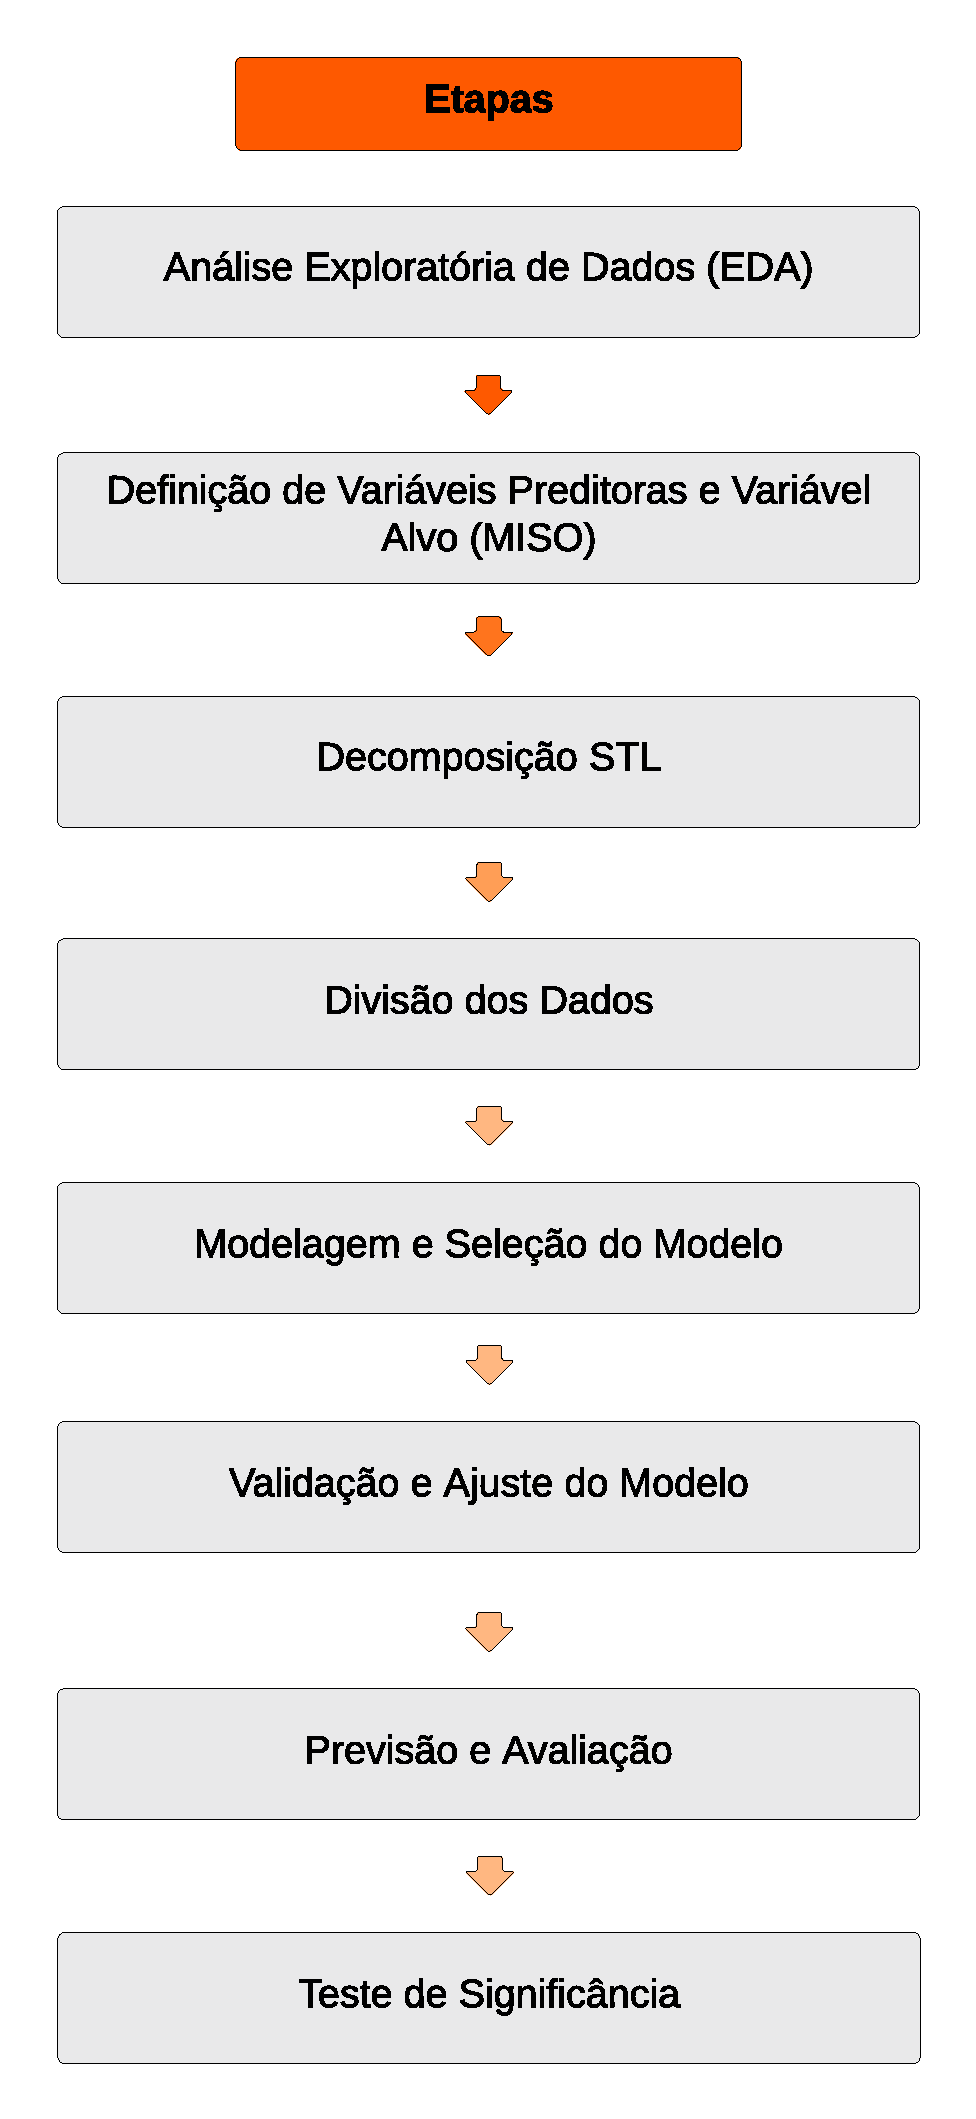
\includegraphics[width=0.4\linewidth]{Introducao/Figuras/Etapas}
	
	
\end{figure}

\noindent As etapas da pesquisa incluem:
\begin{enumerate}[start=1, label={\textbf{Etapa} \arabic*}]
	
	\item \label{etp:1} \textbf{Análise Exploratória de Dados (EDA)}: Nesta etapa  tem-se a identificação de valores ausentes, a observação de padrões temporais e a detecção de anomalias. Gráficos de linha são comuns para visualizar a convergência dos dados \cite{Rostam2021108249}.
	
	\item \label{etp:2} \textbf{Definição de Variáveis Preditoras e Variável Alvo (MISO)}: Na segunda etapa, as variáveis preditoras e a variável alvo para a previsão de Múltiplas Entradas e Uma Saída (do inglês\textit{ Multiple Inputs Single Output}, MISO) são selecionadas. Diferentes modelos, podem incorporar variáveis exógenas na modelagem. Essas variáveis exógenas aprimoram as capacidade de previsão do modelo, especialmente quando o horizonte de previsão se estende além dos dados históricos \cite{PAWLOWSKI202298}. 
	
	\item \label{etp:3} \textbf{Decomposição STL}: O método de decomposição STL (do inglês \textit{Seasonal and Trend Decomposition Using locally estimated scatterplot smoothing (Loess)}) separa uma série temporal em três componentes: sazonalidade, tendência e resíduo. Essa decomposição permite. Decompor séries temporais em sazonal captura variações periódicas e repetitivas. Decompor séries temporais em tendência reflete a evolução geral dos dados ao longo do tempo. Já a componente de resíduo engloba as variações não explicadas pelas anteriores \cite{Bandara2021}.
	
	\item \label{etp:4} \textbf{Divisão dos Dados}: É prática comum dividir o conjunto de dados em conjuntos de treinamento, validação e teste para avaliar o desempenho do modelo. Essa divisão permite uma análise da capacidade de generalização dos modelos, evitando problemas de ajuste excessivo ou insuficiente. A proporção de alocação pode variar, mas uma abordagem é alocar 70\% para treinamento e validação, e os 30\% restantes para o conjunto de testes. A porção de treinamento e validação pode ser subdividida em 80\% para treinamento e 20\% para validação \cite{Tao2020}.
	
	\item \label{etp:5} \textbf{Modelagem e Seleção do Modelo}: Nesta etapa, diversos modelos são construídos e avaliados. Alguns modelos comumente usados para previsão de séries temporais incluem ARX (do inglês \textit{Auto-Regressive with Exogenous Inputs}), AR (do inglês \textit{Auto-Regressive}), MA (do inglês \textit{Moving Average}), ARIMA, SARIMA (do inglês \textit{Seasonal Auto-Regressive Integrated Moving Averages}), SARIMAX (ARIMA Sazonal com variáveis exógenas) e modelos de aprendizado de máquina como RNN, LSTM (do inglês \textit{Long Short-Term Memory}), GRU (do inglês \textit{Gated Recurrent Unit}), Transformer (Transformador), DTR (do inglês \textit{Decision tree regressor}), LR (do inglês \textit{Linear Regression}), XGBoost (do inglês \textit{eXtreme Gradient Boosting}), Light GBM (do inglês \textit{Light Gradient Boosting Machine}) além do Prophet. A escolha do modelo baseia-se em critérios como desempenho na validação, simplicidade do modelo e interpretabilidade dos resultados.
	
	\item \label{etp:6} \textbf{Validação e Ajuste do Modelo}: Durante a construção do modelo, é importante avaliar seu desempenho usando dados de validação. Neste contexto, métricas de avaliação tais como de avaliação como MAE (Erro Médio Absoluto), sMAPE (Erro Médio Percentual Absoluto Simétrico) e RRMSE (Raiz do Erro Médio Quadrático Relativo) podem ser usadas para comparar e selecionar o melhor modelo. Além disso, técnicas de ajuste como otimização de hiperparâmetros e refinamento do modelo usando dados de treinamento e validação combinados podem melhorar o desempenho de previsão de séries temporais.
	
	\item \label{etp:7} \textbf{Previsão e Avaliação}: Com o modelo final com os dados de treinamento e validação, é possível fazer previsões para o conjunto de testes, que representa dados futuros não observados. Essas previsões são comparadas com os valores reais correspondentes para avaliar a qualidade e precisão do modelo.
	
	\item \label{etp:8} \textbf{Teste de Significância}: Aplicar os modelos de previsão e fazer comparativo baseado em testes de significância estatística (\textit{Friedman e Nemenjy}).
	
	O teste de Friedman é uma ferramenta estatística não paramétrica utilizada para comparar três ou mais grupos relacionados quando os dados não atendem aos pressupostos da ANOVA. Ele determina se há diferenças significativas entre os grupos. Se a diferença for confirmada, o teste de Nemenyi é frequentemente empregado para realizar comparações múltiplas entre grupos específicos, identificando quais pares são significativamente diferentes após a rejeição da hipótese nula no teste de Friedman. Assim, esses métodos são cruciais quando se deseja comparar múltiplos grupos sem fazer suposições sobre a distribuição dos dados.

	
\end{enumerate}

Cada uma dessas etapas desempenha um papel crucial na pesquisa e no processo de modelagem de séries temporais, contribuindo para a compreensão dos dados, construção e validação dos modelos.




    